\section{Method}
\label{sec:method}
\subsection{Detector and notation}
CFFM-Net extends YOLO26-n. A pair enters as a four-channel tensor, visible BGR and one thermal grey channel, and the thermal channel is repeated to three for its backbone. Two backbones with separate weights, both initialised from COCO-pretrained YOLO26-n, produce feature maps at each pyramid level that the head reads. A fuser at each of those levels combines the visible map $\Fv$ and the thermal map $\Ft$ into one map $Z$ of the same shape, and the stock YOLO26 neck and one-to-one head consume the fused maps. Because the model subclasses the Ultralytics detection model and keeps the loss and validator unchanged, every result below comes from the standard trainer and the standard COCO-style evaluation. Figure~\ref{fig:overall} shows the layout.

Feature maps have $c$ channels and $h\times w$ cells at the level in question. Reliabilities $\rv,\rt\in(0,1)^{h\times w}$ are single-channel maps.

\subsection{Reliability head}
For each level, a head predicts how far each camera can be trusted at each cell from the evidence in both maps:
\begin{equation}
[\rv,\rt]=\sigma\!\Big(W_r\,\phi\big([\Fv,\;\Ft,\;|\Fv-\Ft|]\big)\Big),
\end{equation}
where $\phi$ is a depthwise $3{\times}3$ convolution with batch normalisation and SiLU, $W_r$ is a $1{\times}1$ convolution to two channels, and $\sigma$ is the logistic function. $W_r$ starts at zero weight with a bias of \cfgInitBias{}, so both cameras are trusted at initialisation. An optional sensor flag $f\in\{0,1\}^2$ per sample multiplies the output, which is how an external monitor can declare a camera dead: the flag forces that camera's reliability to zero everywhere.

\subsection{Offset alignment}
Thermal and visible images are registered in LLVIP but not perfectly in the field. Before the scan, a small convolutional head predicts a two-channel displacement $\Delta=\delta_{\max}\tanh(g([\Fv,\Ft]))$ with $\delta_{\max}=\cfgMaxDisp{}$ cells, and bilinear sampling resamples the thermal map at the displaced positions, giving $\tilde F^{\theta}$. The output layer of $g$ starts at zero, so the block starts as the identity warp and learns a shift only if the loss rewards it.

\subsection{Reliability-gated cross scan}
Both maps are projected to $d=\max(16,\mathrm{round}(\cfgRatio{}\,c))$ channels by a $1{\times}1$ convolution followed by a depthwise $3{\times}3$ convolution, giving $p^{v}$ and $p^{\theta}$. At every cell the visible and thermal tokens are placed next to each other, so a sequence of $L=2hw$ tokens alternates $p^{v}_1,p^{\theta}_1,p^{v}_2,p^{\theta}_2,\dots$ over the raster order. The block scans this sequence in $K=\cfgDirections{}$ orders: rows forward and backward, columns forward and backward. For one direction, token $u_\ell$ with modality $m(\ell)\in\{v,\theta\}$ and grid position $\mathrm{pos}(\ell)$, the recurrence is
\begin{align}
\Delta_\ell &= \softplus\!\big(W_\Delta u_\ell + b_\Delta\big)\,\cdot\, r^{m(\ell)}_{\mathrm{pos}(\ell)},\\
h_\ell &= e^{\Delta_\ell A}\, h_{\ell-1} + \Delta_\ell\, B_\ell\, u_\ell,\\
y_\ell &= C_\ell\, h_\ell + D\, u_\ell,
\end{align}
with $A$ a diagonal matrix of negative entries (state size \cfgDState{}), and $B_\ell$, $C_\ell$ and the pre-activation of $\Delta_\ell$ produced from the token by learned projections, as in Mamba~\cite{gu2023mamba}. The only change from a standard selective scan is the last factor in the first line, the reliability at the token's position for the token's own camera. When that reliability is zero, $\Delta_\ell=0$, the decay factor is one, the input term vanishes, and the state passes the token untouched. A camera with zero reliability therefore cannot alter what the scan carries forward. The outputs of the four directions are mapped back to the grid and summed (Fig.~\ref{fig:scan}).

\begin{figure}[t]
\centering
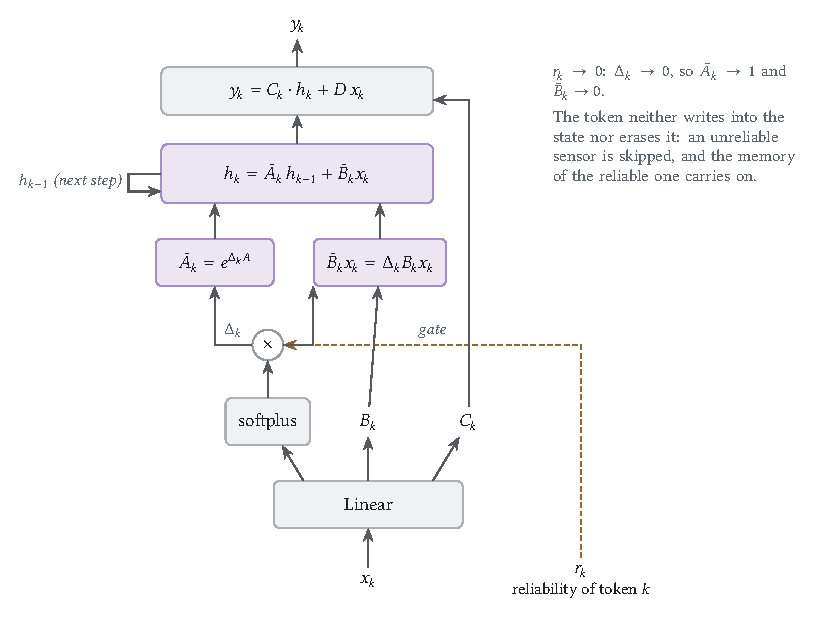
\includegraphics[width=0.8\columnwidth]{figures/fig_gated_scan.pdf}
\caption{One step of the gated scan. The reliability of the token's camera multiplies the step $\Delta_k$ before it enters the decay and the input term, so a reliability near zero leaves the state unchanged.}
\label{fig:scan}
\end{figure}

\subsection{CMFM and fusion levels}
The Cross-Modal Fusion Mamba block (CMFM) wraps the scan with two further paths. The scanned outputs of both modalities are concatenated and normalised by a channel LayerNorm. A local branch applies a depthwise $3{\times}3$ convolution to the concatenation of $p^{v}$ and $p^{\theta}$ and restores the two-dimensional neighbourhood that a one-dimensional scan weakens. A $1{\times}1$ convolution on the concatenation of both paths gives a residual $M$, and the block outputs
\begin{equation}
Z=\frac{\rv\,\Fv+\rt\,\tilde F^{\theta}}{\max(\rv+\rt,\,\cfgWeightFloor{})}+M.
\end{equation}
The projection producing $M$ starts at zero, so a freshly built block is exactly a reliability-weighted average of the two maps, and the scan has to earn any change. The weight floor keeps the gradient of the quotient bounded when both reliabilities approach zero. The scan runs in single precision.

The cost of the scan grows linearly in the number of cells, the number of directions, the channel width and the state size, and it is sequential along each of the $2hw$ tokens, which is why the stride-4 level is excluded from it. 

Figure~\ref{fig:cmfm} shows the block. The detector fuses at the strides that its head reads. In the first version (v1) this is four levels: a reliability-weighted average at stride 4, where a scan over $2hw$ tokens is expensive and buys little, and CMFM at strides 8, 16 and 32. Versions v2 and v3 read the head at strides 8, 16 and 32 only. The baseline replaces every fuser by concatenation followed by a $1{\times}1$ convolution that squeezes the channels back to $c$, the usual two-stream design.

\begin{figure}[t]
\centering
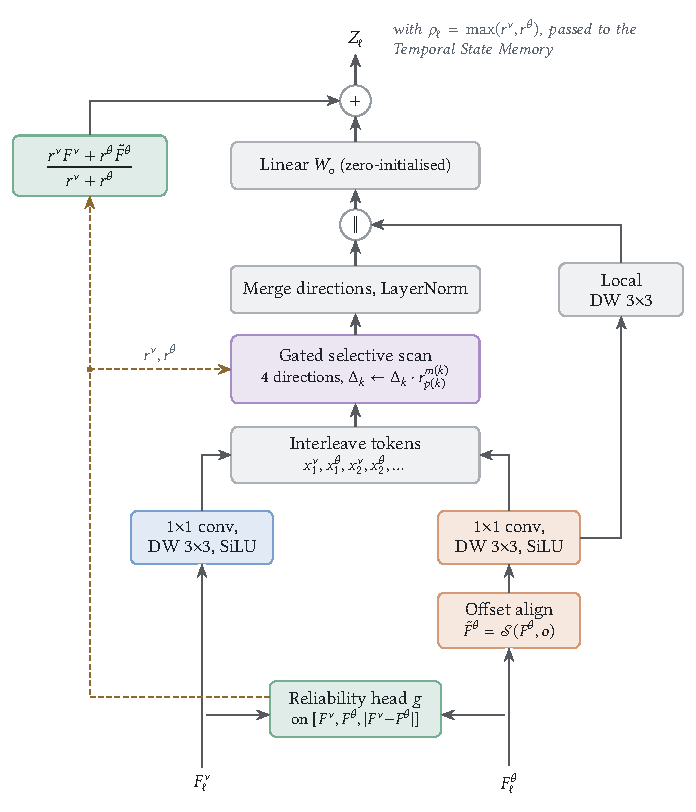
\includegraphics[width=0.78\columnwidth]{figures/fig_cmfm.pdf}
\caption{The CMFM block. A reliability head weights each camera, thermal features are warped onto the visible grid, visible and thermal tokens are interleaved and scanned in four directions with the step scaled by reliability, and a local convolution branch joins before a zero-initialised projection. The result adds to a reliability-weighted average. The larger of the two reliabilities is also passed to the temporal memory.}
\label{fig:cmfm}
\end{figure}

\subsection{Training recipes}
\label{sec:recipes}
Three recipes are compared; they differ in head layout and in what the training batches look like.
\begin{itemize}
\item \textbf{v1.} Four fusion levels, clean pairs only. It is the round-one model.
\item \textbf{v2.} Three levels and \emph{modality dropout}: each training pair has probability \cfgMdProb{} of having its visible camera blacked out, and the same probability for the thermal camera. For half of the blacked-out samples the model also receives the sensor flag. The control baseline is trained with the same dropout, so the comparison isolates the fuser.
\item \textbf{v3.} v2 plus \emph{fault training} and a \emph{reliability loss}. With probability \cfgFaultProb{} a sample has one random camera corrupted by one of the faults of the benchmark below at a random severity, and the head receives a trust target for that camera of \cfgTrustOne{}, \cfgTrustTwo{} or \cfgTrustThree{} at severity one, two or three, and zero for a blacked-out camera (healthy cameras have target one). The reliability loss is the binary cross-entropy between the mean reliability of each gated fuser and its trust target, averaged over fusers and added with weight \cfgRelWeight{}. The ablation \emph{v3 without reliability branch} keeps the fault training and removes the loss; the \emph{fault-trained concat} baseline keeps the fault training and the concat fuser.
\end{itemize}

\subsection{Temporal State Memory}
\label{sec:tsm}
A still-image detector forgets a pedestrian the moment its thermal camera drops a frame. The Temporal State Memory (TSM) gives each fusion level a per-pixel recurrent state that survives across frames. It is attached after the fuser at each level with a residual path that starts at zero, so a model with a fresh memory produces exactly the detections of the model without it (Fig.~\ref{fig:tsm}).

At frame $t$ the fused map $Z_t$ at one level is projected to $c_s=\mathrm{round}(\cfgMemRatio{}\,c)$ channels, $u_t=W_u Z_t$, and every channel at every cell keeps a state of size \cfgMemState{}. The update is a selective scan in time rather than space:
\begin{align}
\delta_t &= \softplus(W_\delta u_t)\cdot\frac{\tau_t}{\tau_0}\cdot\rho_t,\\
S_t &= e^{\delta_t A}\odot \mathcal{W}_{H_t}(S_{t-1}) + \delta_t\, B_t\, u_t,\\
y_t &= C_t\, S_t + D\, u_t,\qquad Z'_t = Z_t + W_o\,\mathrm{DW}(y_t),
\end{align}
where $B_t$ and $C_t$ come from $u_t$ by a $1{\times}1$ convolution, $\mathrm{DW}$ is a depthwise $3{\times}3$ convolution spreading the readout to neighbours, and $W_o$ is zero-initialised. Three factors act on the step. The ratio $\tau_t/\tau_0$ of the real time gap since the previous frame to a nominal gap $\tau_0=\cfgTauZero{}$\,s makes the decay depend on elapsed time, so a stalled camera that returns after a long gap forgets in proportion. The reliability $\rho_t=\max(\rv_t,\rt_t)$ from CMFM is high when at least one camera is trusted, and a frame in which neither camera is reliable writes little into the state. The warp $\mathcal{W}_{H_t}$ resamples the previous state under the homography $H_t$ from frame $t-1$ to $t$, with zeros for newly exposed cells, so the memory follows a moving camera rather than smearing. A scene cut, or a time gap beyond \cfgResetS{}\,s in the live runtime, resets the state.

The memory is trained with the detector frozen. Clips of \cfgClipLen{} frames at stride \cfgClipStride{} are drawn from KAIST training sequences~\cite{hwang2015kaist}, with labels for every frame. With probability one half a clip receives a fault, one of drop, darkness, noise, glare or shift, starting at a random frame and lasting to the end of the clip, which is the situation the memory exists for. The loss is the detection loss averaged over the frames of the clip, backpropagated through time, optimised with AdamW under a one-cycle schedule, with gradient clipping and with any non-finite step skipped.

\begin{figure*}[t]
\centering
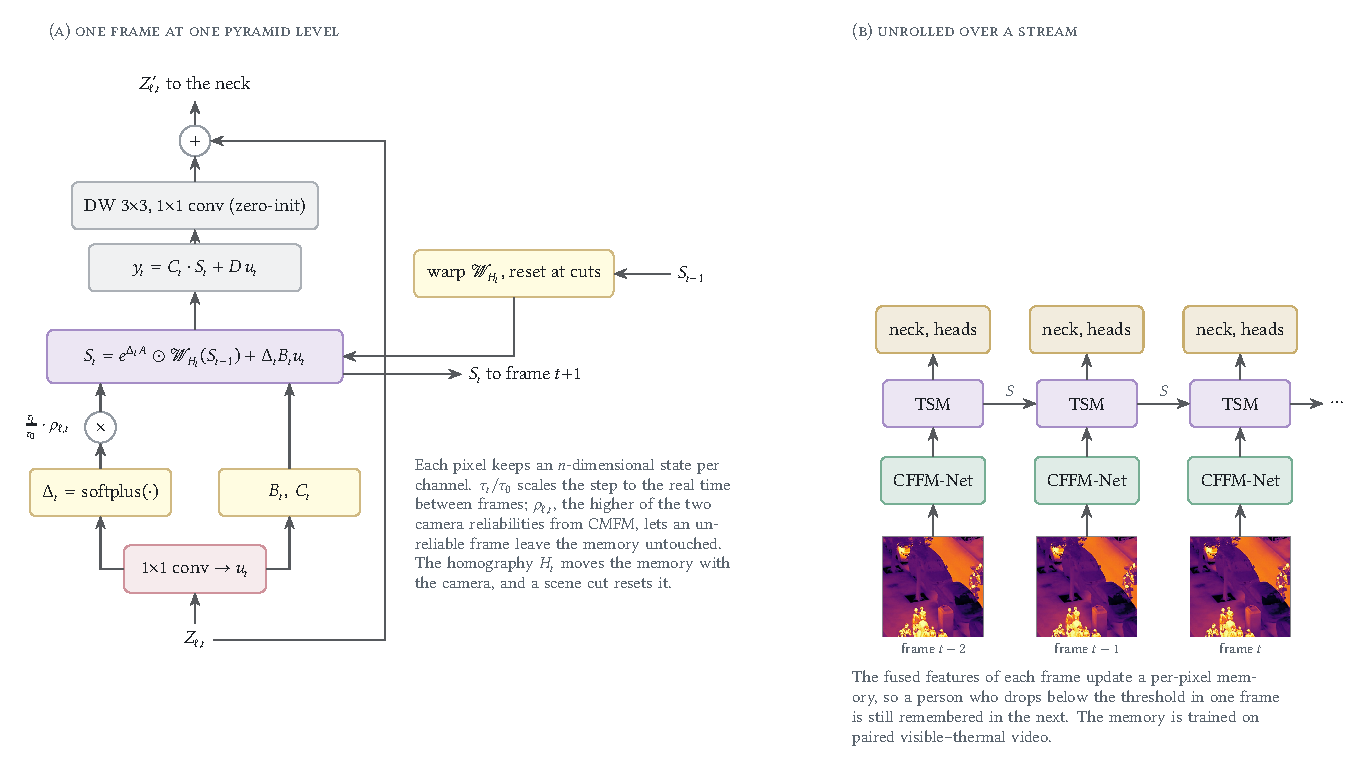
\includegraphics[width=0.82\textwidth]{figures/fig_tsm.pdf}
\caption{The Temporal State Memory. (a) One level at one frame: the step is scaled by elapsed time and by the camera reliability, and the previous state is warped by the frame-to-frame homography. (b) Unrolled over a stream, the memory sits between the fusion output and the neck.}
\label{fig:tsm}
\end{figure*}

\subsection{Causal inference and tracking on video}
\label{sec:causal}
Video inference is causal: frames are processed in order, the state is reset at the start of each sequence, and no future frame is used. For tracking, detections above a low confidence threshold feed ByteTrack~\cite{zhang2022bytetrack}, which also associates low-score boxes with existing tracks. Because the memory affects detections only, switching it off at test time gives the same model without memory, which is the ablation for video.  Detection is scored on KAIST by the log-average miss rate in the standard reasonable setting, split into day, night, failed and healthy frames, and tracking is scored by MOTA, IDF1 and identity switches against the KAIST person tracks.

\subsection{Live runtime}
\label{sec:live}
The live runtime turns the model into a process that reads two cameras and keeps running when they misbehave.

\paragraph{Capture}
Each camera runs in its own thread, stamps every frame with a monotonic time at the moment of capture, and writes it into a one-slot queue. A put replaces the frame waiting there and counts it as dropped, so a slow consumer never builds a backlog and latency cannot grow with time. A source that fails is reopened with backoff. Sources are a webcam, an RTSP stream, or a replay of a recorded sequence at real speed with injected link faults.

\paragraph{Health monitor}
A monitor watches each camera from arrival times and pixels. It declares a camera stalled when no frame has arrived for \cfgStallIntervals{} nominal frame intervals, frozen when a downsampled frame has stayed nearly unchanged for \cfgFreezeFrames{} consecutive frames, black when the mean intensity is near zero, and saturated when a large share of pixels sits at the top of the range. Stalled, frozen and black cameras are \emph{down}, a saturated camera is \emph{degraded}, and others are \emph{ok}. The nominal rate is \cfgNominalFps{} frames per second.

\paragraph{Inference loop}
Each step takes the newest visible frame, waiting at most one frame interval, and the newest thermal frame without waiting, and reuses the last frame of a camera that has produced none. A camera that is down contributes a zero image and a zero sensor flag, which forces its reliability to zero everywhere, so the detector sees the failure as a stated fact rather than inferring it from a black picture. The gap between the timestamps of consecutive newest frames sets $\tau_t$ for the memory, and a gap longer than \cfgResetS{}\,s resets it. The model runs under half precision, followed by ByteTrack. Each step records inference time, end-to-end time from capture of the newest frame to the end of tracking, the time gap, the offset between the two camera timestamps, the health of each camera and the allocated GPU memory.


